%LTeX: language=de-DE
\chapter{Auswertung}
% \section{Problem}
% Wenn ein Koordinatenpunkt aufgenommen werden will, gibt es mehrere Probleme auf die man stößt.

% Zum einen kann nicht gleichzeitig die X und Y Komponente der Koordinate bestimmt werden. Dies muss nacheinander folgen.
% Grund hierfür ist dem Aufbau des Touchscreens geschuldet.

% Bei der Inbetriebnahme wird sich noch ein weiteres Problem ergeben.
% Falls der Touchscreen nicht betätigt wird, gibt der Mikrocontroller trotzdem Werte aus.
% Dabei handelt es sich um Werte, die keinen Sinn ergeben und die Steuerung der Maus z.B. bei einer Ruhephase stören würden.

% Bei einer Messreihe kann es vereinzelt zu einem Wertesprung kommen. 
% Dieses Problem ist der Messunsicherheit des Systems geschuldet. 
% Diese Sprünge gilt es aus der Messreihe heraus zu filter und zu glätten.

% \section{Lösungsansatz}
% Um das Problem, bei einer nicht Betätigung des Touchscreens, zu lösen, soll vor einer Aufnahme von Koordinatenwerte geprüft werden, ob der Touchscreen betätigt wird.
% Ist dies der Fall, so soll die Messung durchgeführt werden.




Um eine Aussage über die Qualität des Touchscreen treffen zu können, werden mehrere Untersuchungen angestellt.

Bei der ersten Untersuchung wird auf die Mitte des Touchscreen gedrückt und die Position wird für eine gewisse Zeit gehalten.
Die Daten werden anschließen ausgewertet (siehe \cref{ab:genau}).

Um die erste Untersuchung zu erweitern wird nun die Mitte des Touchscreen wiederholt gedrückt.
Hierbei soll die Wiederholbarkeit eines Punktes auf dem Touchscreen untersucht werden.
Die Auswertung ist in \cref{ab:wiederholung} zu finden.

Bei der letzten Untersuchung wird die Linearität des Touchscreen untersucht.
Hierfür gibt der Hersteller eine Garantie, unter der sich die Linearität des Touchscreen befinden soll.
Den Wert der angegeben wird liegt bei \SI{1,5}{\%} (siehe \cref{ds:touch} Seite 3 des Datenblatts).

Um die nachfolgende Untersuchungen korrekt durchführen zu können muss zu nächst der Reaktionsbereich des Touchscreens ermittelt werden.
Durch seine Bauform hat dies einen Randbereich, an dem es nicht zuverlässig Werte ausgibt.
Umkehrschluss, das Programm erkennt nicht das etwas den Touchscreen betätigt.
Im Datenblatt werden Werte für den Bereich genannt, in dem es zuverlässig arbeitet.
In X-Richtung hat der Touchscreen einen Arbeitsbereich von \SI{214,5}{mm} und in Y-Richtung einen Bereich von \SI{161,0}{mm}.
Diese Werte wurden durch Messungen ermittelt.

Durch Ausprobieren wurden die maximal und minimal ADC-Werte in die jeweilige Richtung ermittelt.


\begin{table}[h]
    \centering
    \caption[Empirisch ermittelter Wertebereich der ADC]{Empirisch ermittelter Wertebereich der ADC für die äußeren Grenzen des Touchscreens in jeweils horizontaler (x) und vertikaler (y) Richtung.}
    \begin{tabular}{@{}lrr@{}}
        \toprule
            &Min    &Max\\
        \midrule
        x   &68     &961\\
        y   &108    &917\\
        \bottomrule
    \end{tabular}
    \label{tab:ADC min max}
\end{table}

Mit diesen Werten lässt sich Arbeitsbereich (in ADC-Werten) des Touchscreen in jede Richtung bestimmen.
\begin{align}
    ADC_{x,len} &= 961 - 68 = 893
    \label{eq:adcxlen}\\
    ADC_{y,len} &= 917 - 108
    \label{eq:adcylen}
\end{align}
Mittels dieser Werte (\cref{eq:adcxlen} und \cref{eq:adcylen}) können sie im Anschluss in das metrische System überführt werden und die Auflösung des Touchscreen bestimmt werden.
In x-Richtung ergibt sich eine Auflösung von \SI{0,240}{\frac{mm}{ADC}} und in y-Richtung \SI{0,199}{\frac{mm}{ADC}}.

Die unterschiedlichen Werte haben den Ursprung, dass die ADC-Werte sich in x-Richtung auf eine größere Distanz verteilen als in y-Richtung.

\section{Genauigkeit bei konstanten Koordinaten}
\label{ab:genau}
Bei dieser Untersuchung wurden zwei separate Messungen durchführen.
Im ersten Durchlauf wurden die Werte mit dem Medianfilter verarbeitet, bevor sie ausgegeben wurden.
Im zweiten Durchlauf wurden die direkten und ungefilterte Werte ausgegeben.
In den \cref{fig:filtered} und \cref{fig:unfiltered} sind die Messdaten der x- und y-Komponenten aufgetragen (siehe Seite \cref{fig:filtered}).

Die Auswertung der Messdaten ist in \cref{tab:genaufilter} und \cref{tab:genauunfilter} zu finden.
Bei der Auswertung ist zu beachten, dass es um zwei separate Messreihen handelt.
Daher hat auch die ungefilterte Messreihe eine Standardabweichung und Varianz von null, im Vergleich zur gefilterten Messreihe.
Im Normalbetrieb ist der Medianfilter im Programm aktiv, daher haben die Werte der gefilterten Messreihe eine höhere Relevanz.
Die Genauigkeit des Touchscreen in beiden Messreihen ist kleiner als die Auflösung, was auf ein akkurat arbeitenden Touchscreen schließen lässt.
\begin{table}[ht!]
    \caption{Auswertung der gefilterten Messdaten }
    \begin{center}
        \begin{tabular}{@{}lrrrrrr@{} }
            \toprule&\multicolumn{2}{c}{Median}& \multicolumn{2}{c}{Standardabweichung}&\multicolumn{2}{c}{Varianz} \\ 
            Einheit    &(ADC)              &mm             &(ADC)          &mm             &(ADC)      &mm\\\midrule
            x-Richtung & \SI{499,0}{}      & \SI{119,861}{}&\SI{0,0}{}     &\SI{0,0}{}     &\SI{0,0}{} & \SI{0,0}{} \\  
            y-Richtung & \SI{509,999}{}    & \SI{101,495}{}&\SI{0,049}{}   &\SI{0,010}{}   &\SI{0,0}{} & \SI{0,0}{} \\ \bottomrule
        \end{tabular}
        \label{tab:genaufilter}
    \end{center}   
    \caption{Auswertung der ungefilterten Messdaten}
    \begin{center}
        \begin{tabular}{@{}lrrrrrr@{} }
            \toprule&\multicolumn{2}{c}{Median}& \multicolumn{2}{c}{Standardabweichung}&\multicolumn{2}{c}{Varianz} \\ 
            Einheit    &(ADC)              &mm             &(ADC)          &mm             &(ADC)      &mm\\\midrule
            x-Richtung & \SI{499,0}{} & \SI{119,861}{}&\SI{0,0}{}&\SI{0,0}{}&\SI{0,0}{} & \SI{0,0}{} \\  
            y-Richtung & \SI{510,0}{} & \SI{101,496}{}&\SI{0,0}{}&\SI{0,0}{}&\SI{0,0}{} & \SI{0,0}{} \\ \bottomrule
        \end{tabular}
        \label{tab:genauunfilter}
    \end{center}   
\end{table}


\begin{figure}[ht!]
    \centering
    %\includesvg[width=\linewidth]{fig/plots/filtered}
    \caption{Darstellung der gefilterten Messreihe}
    \label{fig:filtered}
    \centering
    %\includesvg[width=\linewidth]{fig/plots/unfiltered}
    \caption{Darstellung der ungefilterten Messreihe}
    \label{fig:unfiltered}
\end{figure}

\newpage

\section{Wiederholbarkeit von Koordinaten}
\label{ab:wiederholung}
Um die Wiederholbarkeit von Koordinaten zu untersuchen, wurde die Mitte des Touchscreen mehrmals berührt während die Messdaten aufgezeichnet wurden.
Die Auswertung der Messdaten sind in \cref{tab:wiederholung} zu sehen.
Aus den Werten kann man sagen, dass die Genauigkeit der Auflösung entspricht.
\begin{table}[ht!]
    \caption{Auswertung der Wiederholbarkeit von Koordinaten}
    \begin{center}
        \begin{tabular}{@{}lrrrrrr@{} }
            \toprule&\multicolumn{2}{c}{Median}& \multicolumn{2}{c}{Standardabweichung}&\multicolumn{2}{c}{Varianz} \\ 
            Einheit    &(ADC)              &mm             &(ADC)          &mm             &(ADC)      &mm\\\midrule
         x-Richtung & \SI{510,75}{}    & \SI{122,683}{}&\SI{0,894}{}   &\SI{0,215}{}   &\SI{0,8}{}     & \SI{0,192}{} \\  
         y-Richtung & \SI{515,858}{}    & \SI{102,661}{}&\SI{1,159}{}   &\SI{0,231}{}   &\SI{1,3}{}     & \SI{0,259}{} \\ \bottomrule 
        \end{tabular}
        \label{tab:wiederholung}
    \end{center}   
\end{table}


\begin{figure}[ht!]
    \centering
    %\includesvg[width=\linewidth]{fig/plots/wiederholung}
    \caption{Darstellung der Wiederholbarkeit von Koordinaten}
    \label{fig:wiederholung}
\end{figure}

\section{Linearität in x- und y-Richtung}
\label{ab:linear}
Um eine Aussage über die Linearität des Touchscreens treffen zu können, wurden in x- und y-Richtung, auf dem Touchscreen alle \SI{10}{mm} eine Markierung gesetzt (siehe \cref{fig:messlinear}).

Die jeweiligen Komponenten wurde anschließend jeweils über die physikalische Strecke in einem Diagramm dargestellt (siehe \cref{fig:xlinear} und \cref{fig:ylinear}).
Die Messwerte wurden mittels einer linearen Anpassung gefittet.

Das \(\chi^2\) gibt Auskunft darüber in welchem Maß Werte miteinander sich verändern.
Je kleiner dieser Wert ist, desto eher stimmt die Linearität überein.
Bei der linearen Anpassung in x-Richtung wurde ein \(\chi^2\) von \(0,294\) ermittelt.
Für die Linearität in y-Richtung wurde ein \(\chi^2\) von \(5,946\) ermittelt.

Bei der Untersuchung, der Linearität in y-Richtung, gibt es bei Abstand 40 mm ein Messpunkt der von der Messpunktewolke und der dazugehörigen linearen Anpassung abweicht. Dieser Messpunkt führt zu diesem größeren \(\chi^2\) als im Vergleich zur Messreihe  in x-Richtung.

Um abschließend eine Aussage treffen zu können, ob diese Werte im Wertebereich des Datenblatts sind (\cref{ds:touch}, \cpageref{ds:touch}), muss der Grenzwert der Chi-Quadrat-Verteilung mit den Werten der linearen Anpassung verglichen werden.
Im Datenblatt wird eine Linearität von \SI{1,5}{\%} garantiert.
In der Wertetabelle von \cite{papula} gibt es nur Werte für \SI{1}{\%} oder \SI{2,5}{\%}.
Der gelistete Wert für zwei Freiheitsgrade und für \SI{1}{\%} liegt bei 7,88.
Sowohl das \(\chi^2\) in x-Richtung wie auch in y-Richtung ist kleiner diesem Werte.
Dies hat zur Folge, dass dieser Touchscreen eine Linearität von unter \SI{1}{\%} aufweist.
% \begin{figure}
%     \begin{minipage}{0.49\linewidth}
%         \centering
%         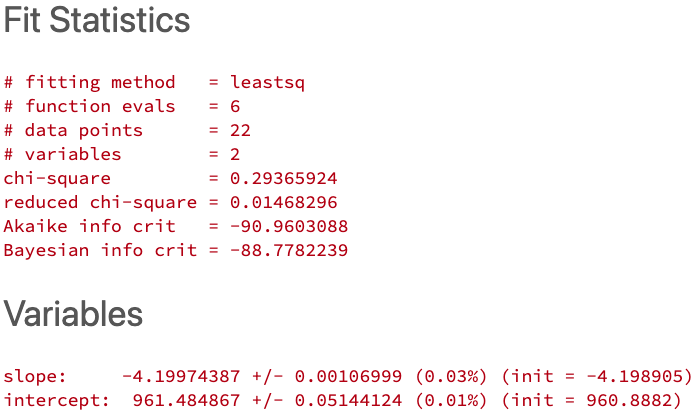
\includegraphics[width=\linewidth]{fig/raster/xfit.png}
%         \caption{Auswertung der Linearität in x-Richtung}
%         \label{fig:xfit}
%     \end{minipage}
%     \begin{minipage}{0.49\linewidth}
%         \centering
%         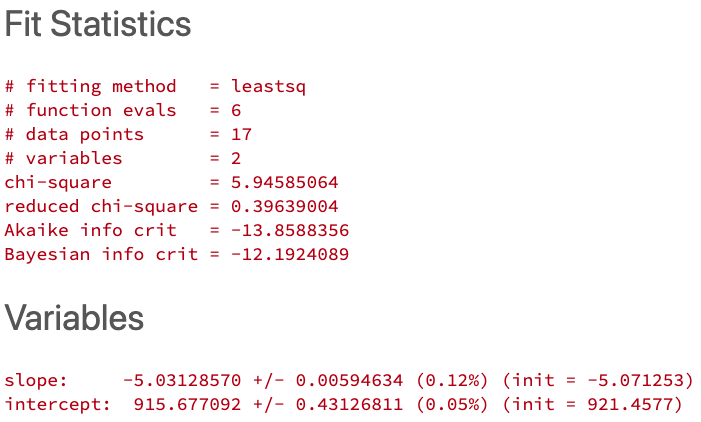
\includegraphics[width=\linewidth]{fig/raster/yfit.png}
%         \caption{Auswertung der Linearität in y-Richtung}
%         \label{fig:yfit}
%     \end{minipage}
% \end{figure} 
\begin{figure}[ht!]
    \centering
    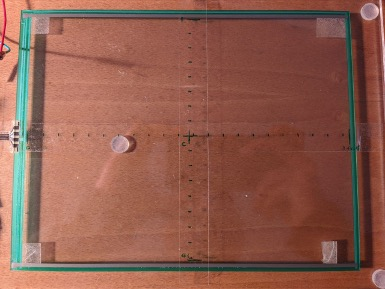
\includegraphics[width=0.6\linewidth]{fig/raster/messlinear.jpg}
    \caption{Messaufbau für Linearität in x- und y-Richtung}
    \label{fig:messlinear}
\end{figure}

\begin{figure}[ht!]
    \centering
    %\includesvg[width=\linewidth]{fig/plots/8_linearitaet_x}
    \caption{}
    \label{fig:xlinear}
    %\includesvg[width=\linewidth]{fig/plots/8_linearitaet_y}
    \caption{}
    \label{fig:ylinear}
\end{figure}
